% Chapter 9, Section 1

\section{The Convolution Operation\index{convolution}\index{cross-correlation}}
\label{sec:convolution}


\subsection*{Intuition}
Convolution extracts local patterns by sliding small filters across the input, producing feature maps that respond strongly where patterns occur. Parameter sharing means the same filter detects the same pattern anywhere, yielding translation equivariance \index{equivariance} and dramatic parameter efficiency \cite{GoodfellowEtAl2016,Prince2023}.

\paragraph{Metaphor: The Detective's Magnifying Glass}
Imagine a detective examining a crime scene photograph with a magnifying glass, systematically scanning every area to look for specific patterns like fingerprints or footprints. The magnifying glass (convolution kernel) is the same tool used everywhere, but it can detect the same type of evidence whether it appears in the top-left corner or bottom-right corner of the photo. This is exactly how convolution works in neural networks—the same learned pattern detector scans across the entire image, finding similar features wherever they appear.

\paragraph{Example: Edge Detection}
Consider a simple edge detection filter that looks for vertical edges in an image. This filter might have values like $[-1, 0, 1]$ for a horizontal line of pixels. When this filter slides across an image, it produces high responses where there are strong vertical edges (like the side of a building) and low responses in flat areas (like the sky). The same filter works identically whether the edge is in the center of the image or near the edges, demonstrating the translation equivariance property that makes CNNs so powerful for image processing.

\begin{figure}[h]
\centering
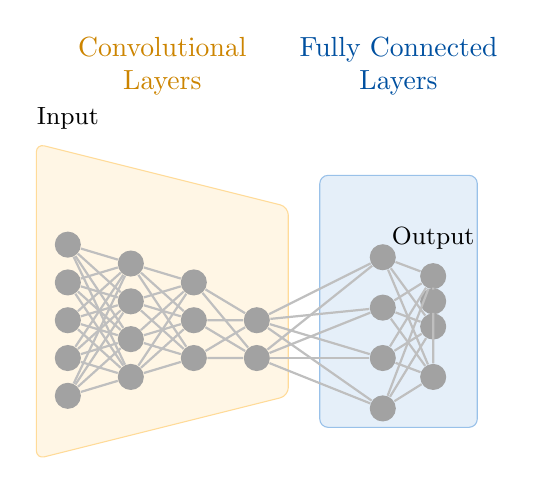
\begin{tikzpicture}[scale=0.8]
  % Define colors
  \definecolor{convcolor}{RGB}{255,165,0}
  \definecolor{fccolor}{RGB}{0,100,200}
  \definecolor{nodecolor}{RGB}{100,100,100}
  
  % Convolutional layers (orange region)
  \draw[convcolor!40,fill=convcolor,fill opacity=0.1,rounded corners=3]
    (0.5,-2.5) -- (0.5,2.5) -- (4.5,1.5) -- (4.5,-1.5) -- cycle;
  
  % Fully connected layers (blue region)
  \draw[fccolor!40,fill=fccolor,fill opacity=0.1,rounded corners=3]
    (5,-2) rectangle (7.5,2);
  
  % Input layer
  \foreach \i in {1,...,5} {
    \node[circle,fill=nodecolor!60,minimum size=0.3cm] (input\i) at (1,{1.5-\i*0.6}) {};
  }
  \node[above=0.3cm] at (1,2.2) {\small Input};
  
  % Convolutional layers
  \foreach \i in {1,...,4} {
    \node[circle,fill=nodecolor!60,minimum size=0.3cm] (conv1\i) at (2,{1.2-\i*0.6}) {};
  }
  \foreach \i in {1,...,3} {
    \node[circle,fill=nodecolor!60,minimum size=0.3cm] (conv2\i) at (3,{0.9-\i*0.6}) {};
  }
  \foreach \i in {1,...,2} {
    \node[circle,fill=nodecolor!60,minimum size=0.3cm] (conv3\i) at (4,{0.3-\i*0.6}) {};
  }
  
  % Fully connected layers
  \foreach \i in {1,...,4} {
    \node[circle,fill=nodecolor!60,minimum size=0.3cm] (fc1\i) at (6,{1.5-\i*0.8}) {};
  }
  \foreach \i in {1,...,3} {
    \node[circle,fill=nodecolor!60,minimum size=0.3cm] (fc2\i) at (6.8,{1.2-\i*0.8}) {};
  }
  
  % Output layer
  \node[circle,fill=nodecolor!60,minimum size=0.3cm] (output) at (6.8,0) {};
  \node[above=0.3cm] at (6.8,0.3) {\small Output};
  
  % Connections (simplified)
  \foreach \i in {1,...,5} {
    \foreach \j in {1,...,4} {
      \draw[gray!50,thick] (input\i) -- (conv1\j);
    }
  }
  
  \foreach \i in {1,...,4} {
    \foreach \j in {1,...,3} {
      \draw[gray!50,thick] (conv1\i) -- (conv2\j);
    }
  }
  
  \foreach \i in {1,...,3} {
    \foreach \j in {1,...,2} {
      \draw[gray!50,thick] (conv2\i) -- (conv3\j);
    }
  }
  
  \foreach \i in {1,...,2} {
    \foreach \j in {1,...,4} {
      \draw[gray!50,thick] (conv3\i) -- (fc1\j);
    }
  }
  
  \foreach \i in {1,...,4} {
    \foreach \j in {1,...,3} {
      \draw[gray!50,thick] (fc1\i) -- (fc2\j);
    }
  }
  
  \foreach \i in {1,...,3} {
    \draw[gray!50,thick] (fc2\i) -- (output);
  }
  
  % Labels
  \node[above=0.5cm,align=center,convcolor!80!black] at (2.5,2.5) {Convolutional\\Layers};
  \node[above=0.5cm,align=center,fccolor!80!black] at (6.25,2.5) {Fully Connected\\Layers};
  
\end{tikzpicture}
\caption{Deep CNN: conv layers (orange) maintain spatial structure, FC layers (blue) process global features.}
\label{fig:deep-cnn-architecture}
\end{figure}

\subsection{Definition}

The \textbf{convolution} operation applies a filter (kernel) across an input:

For discrete 2D convolution:
\begin{equation}
S(i,j) = (I * K)(i,j) = \sum_m \sum_n I(i-m, j-n) K(m, n)
\end{equation}

where $I$ is the input and $K$ is the kernel. In deep learning libraries, the implemented operation is often cross-correlation (no kernel flip).

In practice, we often use \textbf{cross-correlation}:
\begin{equation}
S(i,j) = (I * K)(i,j) = \sum_m \sum_n I(i+m, j+n) K(m, n)
\end{equation}

\subsection{Properties}

The convolution operation possesses several fundamental properties that make it particularly well-suited for processing grid-structured data like images. Parameter sharing represents one of the most important characteristics, where the same kernel is applied across all spatial locations, dramatically reducing the number of parameters compared to fully connected layers acting on flattened images. This parameter sharing yields translation equivariance, meaning that if the input shifts spatially, the feature map shifts in exactly the same way. Formally, letting \(T_\delta\) denote a spatial shift, we have \((T_\delta I) * K = T_\delta (I * K)\) under appropriate boundary conditions, making CNNs robust to object translations in images.\index{parameter sharing}

Local connectivity ensures that each output depends only on a local input region, known as the receptive field, which exploits the spatial locality inherent in natural images where nearby pixels are statistically dependent. This local processing enables compositionality, where stacking layers progressively grows the effective receptive field, allowing the network to detect increasingly complex patterns that build from simple edges to corners to object parts. The linear nature of convolution operations, when combined with pointwise nonlinearities like ReLU, creates the foundation for modeling complex functions while maintaining computational efficiency.\index{receptive field}

Padding and boundary effects play crucial roles in preserving spatial information and mitigating edge shrinkage that occurs when kernels extend beyond image boundaries. Without proper padding, repeated convolutions rapidly reduce feature map size and bias learned features toward the center of the image. Stride and downsampling provide efficient ways to reduce spatial resolution, though aggressive striding early in the network can remove important fine details, leading many modern designs to delay downsampling to later stages. Dilation, or atrous convolutions, offers an alternative approach by inserting holes between kernel elements to increase the receptive field without increasing parameters, proving particularly useful for dense prediction tasks like semantic segmentation.\index{padding}\index{stride}\index{dilation}

The combination of convolution with pooling or global aggregation introduces partial translation invariance in the representation, while multi-channel mixing through kernels of shape \(k\times k\times C_{\text{in}}\) enables learning both spatial and cross-channel interactions. The strategic use of $1\times1$ convolutions allows mixing channels without spatial coupling, serving as bottlenecks and dimension reduction techniques in modern architectures like Inception and ResNet.\cite{GoodfellowEtAl2016,Prince2023,Krizhevsky2012,He2016}

\subsection{Multi-Channel Convolution}

For input with $C_{\text{in}}$ channels and $C_{\text{out}}$ output channels:
\begin{equation}
S_{c_{\text{out}}}(i,j) = \sum_{c_{\text{in}}=1}^{C_{\text{in}}} (I_{c_{\text{in}}} * K_{c_{\text{out}}, c_{\text{in}}})(i,j) + b_{c_{\text{out}}}
\end{equation}

\paragraph{Understanding Multi-Channel Convolution and S(i,j)}
Multi-channel convolution is the fundamental operation that enables CNNs to process complex inputs like RGB images (3 channels) and produce rich feature representations. The notation $S_{c_{\text{out}}}(i,j)$ represents the output feature map value at spatial position $(i,j)$ for output channel $c_{\text{out}}$. This operation allows the network to learn both spatial patterns (through kernel sliding) and cross-channel interactions (by mixing information from different input channels). Each output channel $S_{c_{\text{out}}}(i,j)$ captures how strongly a particular learned pattern is detected at location $(i,j)$, where higher values indicate stronger pattern matches. This enables the network to detect complex features that span across multiple input channels while maintaining spatial locality and translation equivariance.

\subsection{Hyperparameters}

The design of convolutional layers involves several critical hyperparameters that significantly impact both computational efficiency and learning performance. Kernel size represents one of the most fundamental choices, with $3 \times 3$ and $5 \times 5$ kernels being the most common selections in practice. Modern architectures often prefer stacked $3\times3$ convolutions over single $5\times5$ kernels, as demonstrated in VGG networks, because they provide the same receptive field with fewer parameters and better gradient flow.\cite{GoodfellowEtAl2016}

Stride controls the step size for sliding the kernel across the input, directly affecting the spatial resolution of the output feature maps. The relationship between input size, kernel size, and stride determines the output dimensions through the formula $\text{Output size} = \left\lfloor \frac{n - k}{s} \right\rfloor + 1$, where $n$ is the input size, $k$ is the kernel size, and $s$ is the stride. Padding strategies provide different approaches to handling boundary effects, with "valid" padding using no padding, "same" padding preserving spatial size, and "full" padding providing maximum coverage. For "same" padding with stride 1, the required padding is calculated as $p = \left\lfloor \frac{k-1}{2} \right\rfloor$, ensuring that the output maintains the same spatial dimensions as the input.\index{stride}\index{padding}

% \subsection{Visual Aid}
% \begin{figure}[h]
%     \centering
%     % illustrative kernel sliding grid using TikZ
%     \begin{tikzpicture}[scale=0.5]
%         % input grid 5x5
%         \foreach \i in {0,...,5} {\draw (0,\i) -- (5,\i);}
%         \foreach \j in {0,...,5} {\draw (\j,0) -- (\j,5);}
%         % kernel window 3x3 at (1,1)
%         \draw[bookred,very thick] (1,1) rectangle (4,4);
%     \end{tikzpicture}
%     \caption{A $3\times3$ kernel sliding over a $5\times5$ input highlights local pattern extraction.}
%     \label{fig:conv-sliding-window}
% \end{figure}

